% FortySecondsCV LaTeX template
% Copyright © 2019-2020 René Wirnata <rene.wirnata@pandascience.net>
% Licensed under the 3-Clause BSD License. See LICENSE file for details.
%
% Please visit https://github.com/PandaScience/FortySecondsCV for the most
% recent version! For bugs or feature requests, please open a new issue on
% github.
%
% Contributors
% ------------
% * ifokkema
% * Bertbk
% * Hespe
%
% Attributions
% ------------
% * fortysecondscv is based on the twentysecondcv class by Carmine Spagnuolo
%   (cspagnuolo@unisa.it), released under the MIT license and available under
%   https://github.com/spagnuolocarmine/TwentySecondsCurriculumVitae-LaTex
% * further attributions are indicated immediately before corresponding code


%-------------------------------------------------------------------------------
%                             ADDITIONAL PACKAGES
%-------------------------------------------------------------------------------
\documentclass[
	a4paper,
	% showframes,
	% vline=2.2em,
	% maincolor=cvgreen,
	% sidecolor=gray!50,
	% sectioncolor=red,
	% subsectioncolor=orange,
	% itemtextcolor=black!80,
	% sidebarwidth=0.4\paperwidth,
	% topbottommargin=0.03\paperheight,
	% leftrightmargin=20pt,
	% profilepicsize=4.5cm,
	% profilepicborderwidth=3.5pt,
	% profilepicstyle=profilecircle,
	% profilepiczoom=1.0,
	% profilepicxshift=0mm,
	% profilepicyshift=0mm,
	% profilepicrounding=1.0cm,
]{fortysecondscv}

% improve word spacing and hyphenation
\usepackage{microtype}
\usepackage{ragged2e}
%\usepackage{background}

% uncomment in case you don't want any hyphenation
% \usepackage[none]{hyphenat}

% take care of proper font encoding
\ifxetexorluatex
	\usepackage{fontspec}
	\defaultfontfeatures{Ligatures=TeX}
%	\newfontfamily\headingfont[Path = fonts/]{segoeuib.ttf} % local font
\else
	\usepackage[utf8]{inputenc}
	\usepackage[T1]{fontenc}
%	\usepackage[sfdefault]{noto} % use noto google font
\fi

% enable mathematical syntax for some symbols like \varnothing
\usepackage{amssymb}

% bubble diagram configuration
\usepackage{smartdiagram}
\smartdiagramset{
	% default font size is \large, so adjust to harmonize with sidebar layout
	bubble center node font = \footnotesize,
	bubble node font = \footnotesize,
	% default: 4cm/2.5cm; make minimum diameter relative to sidebar size
	bubble center node size = 0.4\sidebartextwidth,
	bubble node size = 0.25\sidebartextwidth,
	distance center/other bubbles = 1.5em,
	% set center bubble color
	bubble center node color = maincolor!70,
	% define the list of colors usable in the diagram
	set color list = {maincolor!10, maincolor!40,
	maincolor!20, maincolor!60, maincolor!35},
	% sets the opacity at which the bubbles are shown
	bubble fill opacity = 0.8,
}


%-------------------------------------------------------------------------------
%                            PERSONAL INFORMATION
%-------------------------------------------------------------------------------
%% mandatory information
% your name
\cvname{Luiz Barbosa}
% job title/career
\cvjobtitle{Signal Processing Engineer,\\[0.2em] Data Scientist}

%% optional information
% profile picture
% \cvprofilepic{pics/profile.png}

% NOTE: ordering in sidebar will mimic the following order
% date of birth
\cvbirthday{08/05/1982}
% short address/location, use \newline if more than 1 line is required
%\cvaddress{Park Ave.~1, 555 555 B-Woods}
% phone number
\cvphone{+55 (61) 981 882 169}
% personal website
%\cvsite{https://pandascience.net}
% email address
\cvmail{contato@luizbarbosa.net}
% pgp key
%\cvkey{4096R/FF00FF00}{0xAABBCCDDFF00FF00}
% any other custom entry
%\cvcustomdata{\faFlag}{Brazilian}

%-------------------------------------------------------------------------------
%                              SIDEBAR 1st PAGE
%-------------------------------------------------------------------------------
% add more profile sections to sidebar on first page
\addtofrontsidebar{
	% include gosquare national flags from https://github.com/gosquared/flags;
	% naming according to ISO 3166-1 alpha-2 country codes
	\graphicspath{{pics/flags/}}
	
	% social network accounts incl. proper hyperlinks
	\profilesection{Social Network}
		\begin{icontable}{2.5em}{1em}
			\social{\flag{linkedin.png}}
				{https://www.linkedin.com/in/luiz-barbosa-4aa79282/}
				{luiz-barbosa-4aa79282}
			\social{\faGithub}
				{https://github.com/lujoba}
				{github.com/lujoba}
		\end{icontable}
	
    \profilesection{About Me}
	\aboutme{
		I work with artificial intelligence techniques for Banco do Brasil's computer vision room.  I work with artificial intelligence techniques for Banco do Brasil’s computer vision room. I have deep knowledge of machine learning and deep learning. I am passionate about signal processing, robotics, and mathematics. In my master’s degree, I also used AI techniques to classify the electrical signal of the forearm in order to move a virtual prosthesis. Now, in my Ph.D., in applied mathematics, I am studying the reconstruction of signals sampled at a sub-Nyquist frequency.
	}

	\profilesection{Skills}
		\pointskill{\faGraduationCap}{Machine Learning}{5}[5]
			\skill[1.8em]{\faCompress}{Clustering, Classification,\\Dimensionality Reduction,\\Regression}
		\pointskill{\faGraduationCap}{Deep Learning}{5}[5]
			\skill[1.8em]{\faCompress}{LSTM, CNN,\\Reinforcement Learning}
		\pointskill{\faGraduationCap}{Data Science}{4}[5]
			\skill[1.8em]{\faCompress}{Pandas, Numpy, Skit-Learn,\\SciPy, JuliaDB}
		\pointskill{\faGraduationCap}{Probability\\and Statistics}{5}[5]
		    \skill[1.8em]{\faCompress}{Stochastic Process, Random Variables, Entropy}
		\pointskill{\faGraduationCap}{Computer Vision}{5}[5]
		    \skill[1.8em]{\faCompress}{openCV, DSP}
		\pointskill{\faGraduationCap}{Tensorflow}{5}[5]
		\pointskill{\faGraduationCap}{PyTorch}{5}[5]

}


%-------------------------------------------------------------------------------
%                              SIDEBAR 2nd PAGE
%-------------------------------------------------------------------------------
\addtobacksidebar{
    \graphicspath{{pics/flags/}}

	\profilesection{Programming}
	    \pointskill{\faChild}{Python}{5}[5]
		\pointskill{\faChild}{C/C++}{3}[5]
		\pointskill{\faChild}{C\#}{3}[5]
		    \skill[1.8em]{\faCompress}{Unity 3D}
		\pointskill{\faChild}{MATLAB}{5}[5]
		\pointskill{\faChild}{Julia}{2}[5]
		    \skill[1.8em]{\faCompress}{flux}

	\profilesection{Languages}
	    \pointskill{\flag{GB.png}}{English}{5}
    	\pointskill{\flag{FR.png}}{French}{2}
    	\pointskill{\flag{JP.png}}{Japanese}{1}
		\pointskill{\flag{DE.png}}{German}{1}

	\profilesection{Interests}
		\skill{\faCompress}{Signal Processing}
		\skill{\faCompress}{Computer vision}
		\skill{\faCompress}{Artificial intelligence}
		\skill{\faCompress}{Robotics}
}


%-------------------------------------------------------------------------------
%                         TABLE ENTRIES RIGHT COLUMN
%-------------------------------------------------------------------------------
\begin{document}

\makefrontsidebar

%\backgroundsetup{
%    placement=center,
%    scale=2,
%    angle=0,
%    opacity=0.7,
%    nodeanchor=center,
%    contents={
%        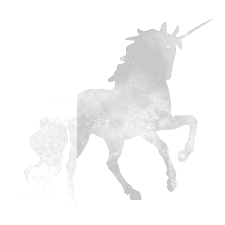
\includegraphics[width=0.8\linewidth]{pics/unicorn2.png}
%    }
%}

\cvsection{Working Experience}
\begin{cvtable}[3]
	\cvitem{Currently}{Researcher in Apllied Mathematics}{University of Brasília, Brasília – DF}
	    {Research of mathematical methods for signal analysis, compression, coding and reconstruction of signals sampled at a sub-Nyquist frequency.}
	\cvitem{2019 -- today}{Data Scientist  and Signal Processing Engineer}{Stefanini TI Solutions, Barsília – DF}
	    {Studies about signal analysis on the time and frequency domain, for video processing and the application of machine learning and deep learning algorithms for Banco do Brasil in computer vision for security (anti-spoofing), facial and finger print recognition.}
    \cvitem{2018 -- 2020}{Researcher in Biomedical Engineering}{University of Brasília, Brasília – DF}
        {Study of the myoelectric signal for the creation of an algorithm for the classification of the electrical signal of the forearm muscles. Through these studies came the understanding for the formalization of an algorithm for the pre-processing of the myoelectric signal. This study led to the creation of a control algorithm for a virtual manual prosthesis in real time.}
    \cvitem{2016 -- 2017}{Project Coordination}{Sotovia Arquitetos Associados, Brasília – DF}
        {Support to the Project Coordination of the Alberto Alcolumbre International Airport - Macapá - AP still working as a facilitator of the teams and Coordinator of the Electronics and Telematics team.}
\end{cvtable}


\cvsection{Education}
\cvsubsection{Postgraduate Training}
\begin{cvtable}[1.5]
	\cvitem{2020 -- today}{PhD degree in Apllied Mathematics}{University of Brasília, Brasília – DF}
		{In-depth studies on mathematical methods for signal analysis, compression, coding and reconstruction of signals sampled at a sub-Nyquist frequency.}
	\cvitem{2018 -- 2020}{Master degree in Biomedical Engineering}{University of Brasília, Brasília – DF}
		{Study of the myoelectric signal for the creation of an algorithm for the classification of the electrical signal of the forearm muscles. Through these studies came the understanding for the formalization of an algorithm for the pre-processing of the myoelectric signal. This study led to the creation of a control algorithm for a virtual manual prosthesis in real time.}
	\cvitem{}{Master Theses}{University of Brasília, Brasília – DF}
		{Use of entropy and clustering for the classification of the myo-eletric signal in combination with the use of machine learning deep learning techniques.}
\end{cvtable}


\cvsubsection{Study}
\begin{cvtable}[1.5]
	\cvitem{2000 -- 2009}{Bachelor in Mechatronics Engineering}{University of Brasília, Brasília – DF}
	{Bachelor degree of mechatronic engineer, with studies in electronics, robotics, programming, control, thermodynamics, resistance of materials.}
\end{cvtable}


\newpage
\makebacksidebar
% \newgeometry{
% 	top=\topbottommargin,
% 	bottom=\topbottommargin,
% 	right=\leftrightmargin,
% 	left=\leftrightmargin
% }

\cvsection{Publications}
\begin{cvtable}
    \cvpubitem{Entropy and Clustering Information Applied to sEMG\\ Classification}
    {42nd Annual International Conferences of the IEEE Engineering in Medicine and Biology Society}{EMBS}{2020}
	\cvpubitem{Image-Based Analisys of Human Tissue Regeneration\\During Therapy Based on Photobiostimulation and\\Natural Latex Biomembranes}
	{Latin American Conference on Biomedical Engineering}
	{CLAIB}{2019}
	\cvpubitem{Simultaneous Myoelectric Pattern Recognition}
	{XXVI Congresso Brasileiro de Engenharia Biomédica}
	{CBEB}{2018}
	\cvpubitem{Exosqueleto Robótico de 4GDL para la Rehabilitación de Miembro Superior}
	{IX Congreso Iberoamericano de Tecnologías de Apoyo a la Discapacidad}
	{IBERDISCAP}{2017}
\end{cvtable}


\cvsection{Extra-Curricular Activities}
\begin{cvtable}
	\cvitemshort{Sport}{Outdoor climbing}
	\cvitemshort{Art}{Photography}
\end{cvtable}

\cvsignature

\end{document}
